\subsection{Explainability Method}
Attention weights were extracted from the model output and visualized as a heatmap to highlight which serialized features contributed most to the prediction. The visualization method corresponds to Figure 3 of the paper.

The aggregated attention scores are visualized as a heatmap, matching Figure~\ref{fig:heatmap}, and presented alongside the LLM output to provide users with interpretable insights into model reasoning.

\begin{figure}[htbp]
    \centering
    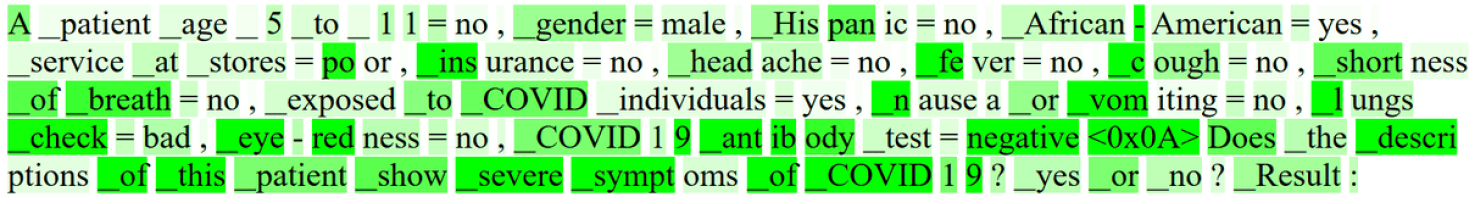
\includegraphics[width=1\textwidth]{fig/fig4.png}
    \caption{The attention map for a predicted positive case where the darker color represents larger attention weights for each token. The prompts are tokenized to mimic the actual inputs to the large language models (LLMs).}
    \label{fig:heatmap}
\end{figure}
